\newcommand{\FigSensMomTransfer}{
\begin{figure}[tb]
\centering 
%\fbox{
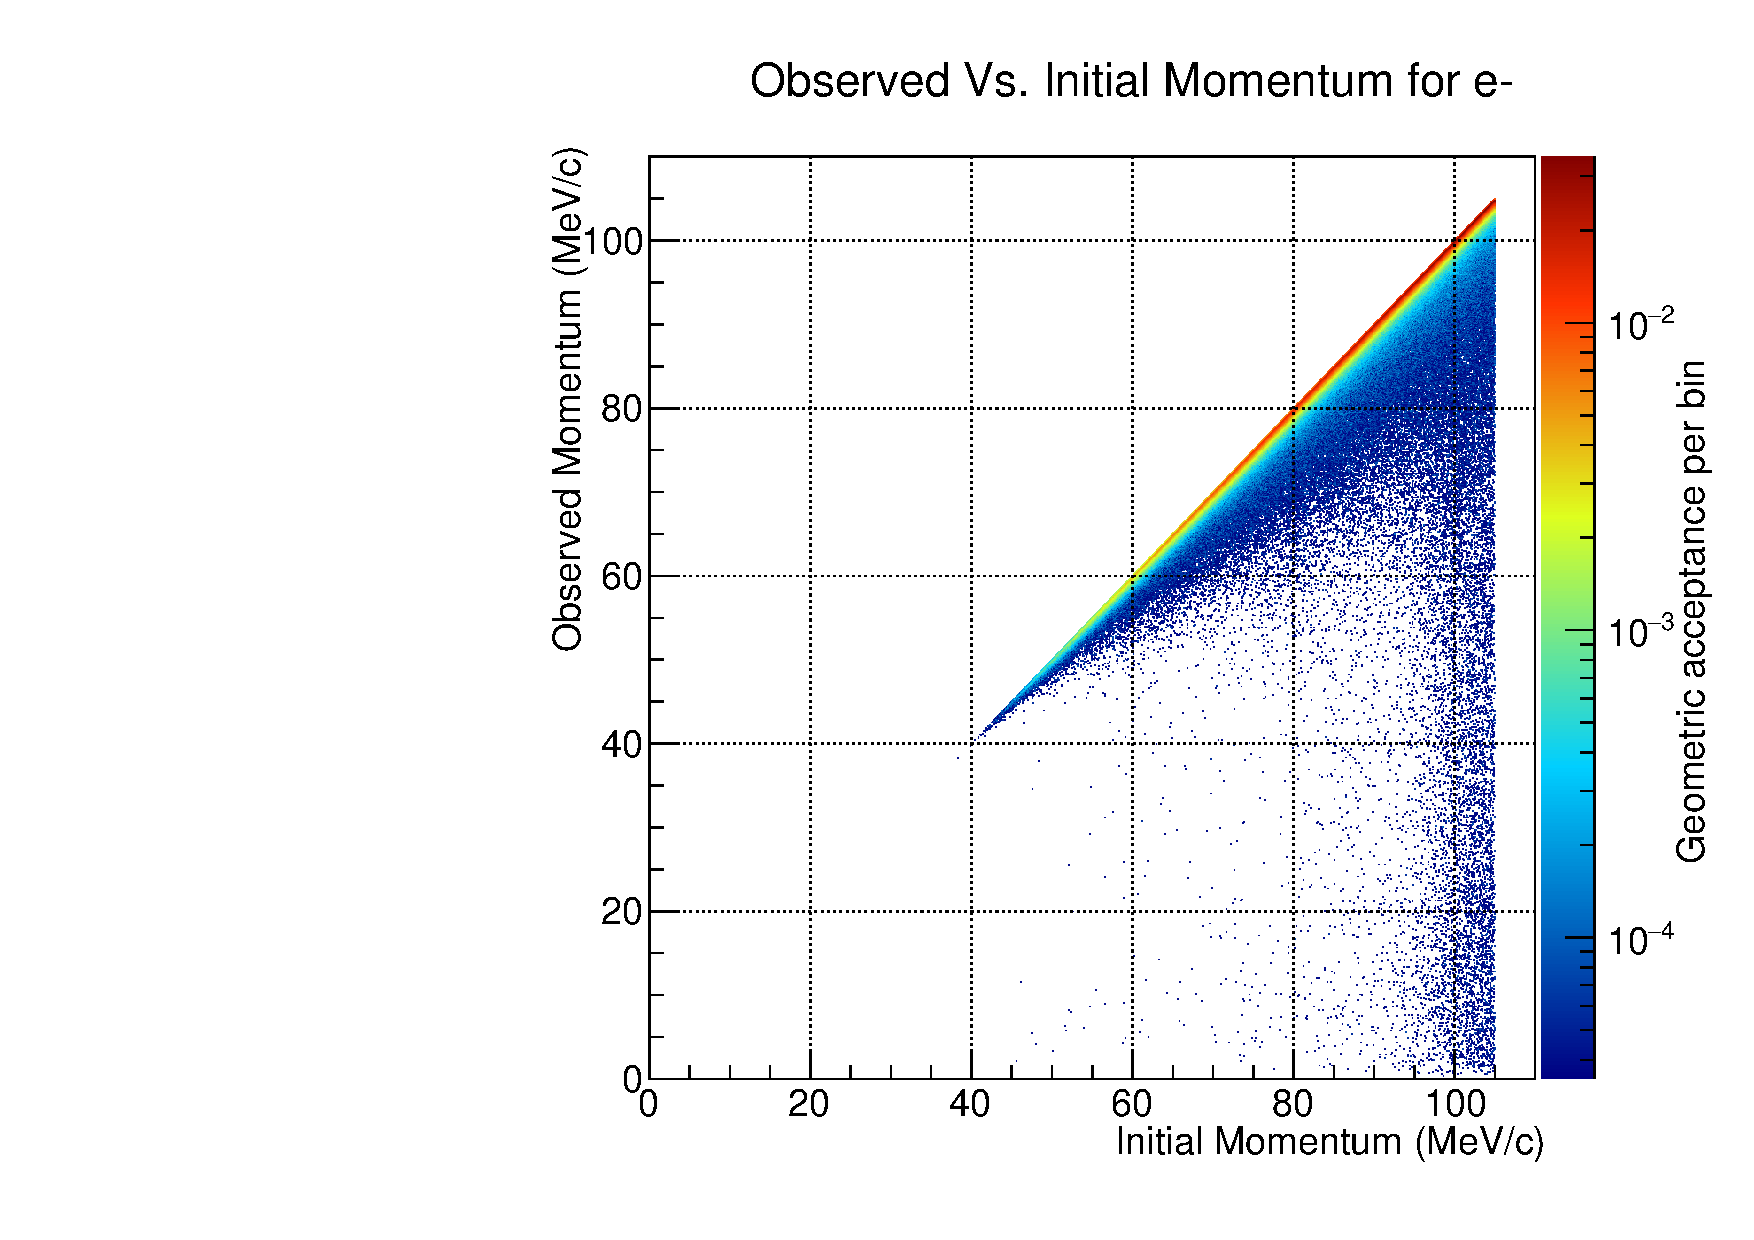
\includegraphics[width=0.5\textwidth,trim=0.0cm 0.0cm 0.0cm 1.6cm,clip]{figs/sensitivity/MomentumTransfer.pdf}
%}
\caption{\figlabel{optim:sense:momTransfer}
The transfer matrix for electrons originating at the target, including the geometric acceptance and energy loss.
}
\end{figure}
}

\newcommand{\FigSensMomSpectra}{
\begin{figure}[tb]
\centering 
%\fbox{
\subfloat[\figlabel{optim:sense:spectra:ELoss}Incl.~energy loss]             {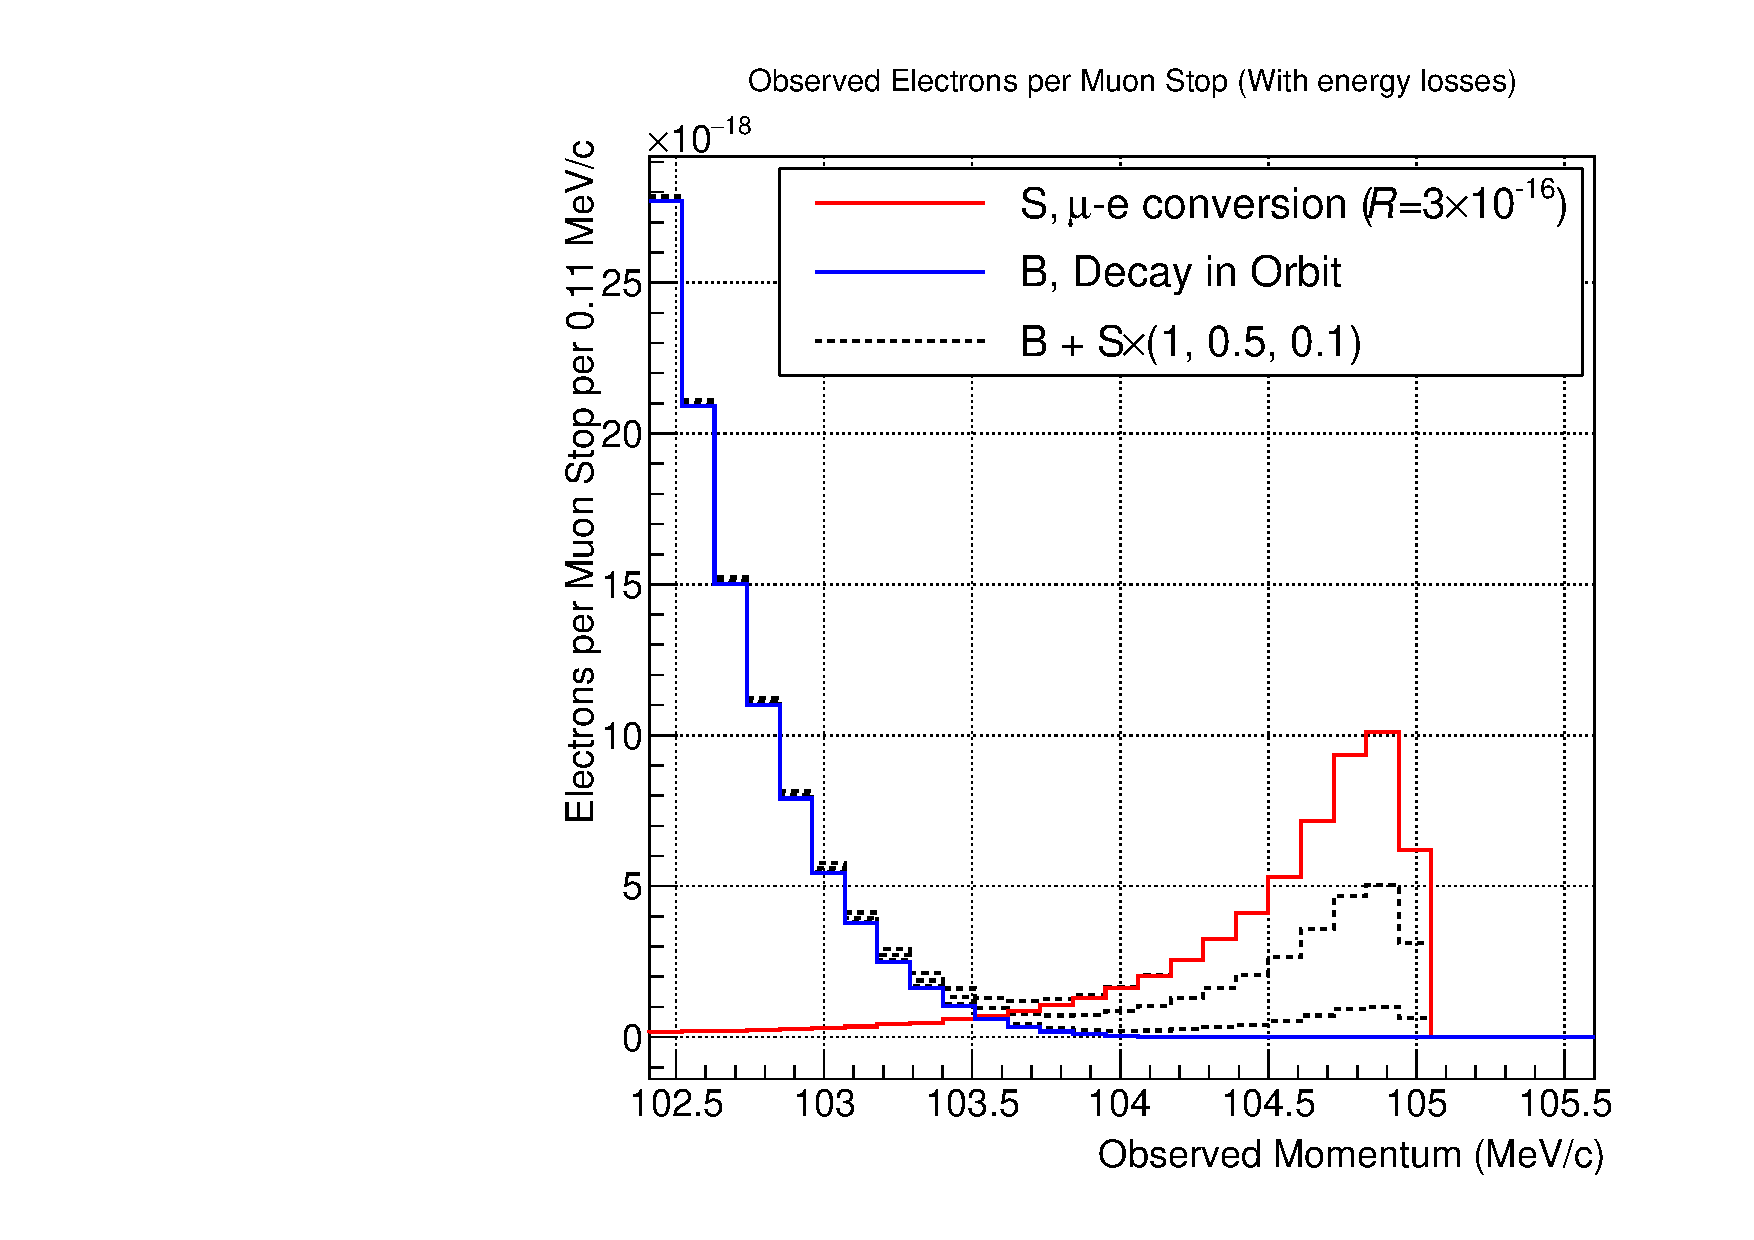
\includegraphics[width=0.48\textwidth,trim=0.0cm 0.0cm 1.0cm 1.0cm,clip]{figs/sensitivity/ConversionVsDio_Spectra.pdf}}
\subfloat[\figlabel{optim:sense:spectra:resolution}Energy loss \& resolution]{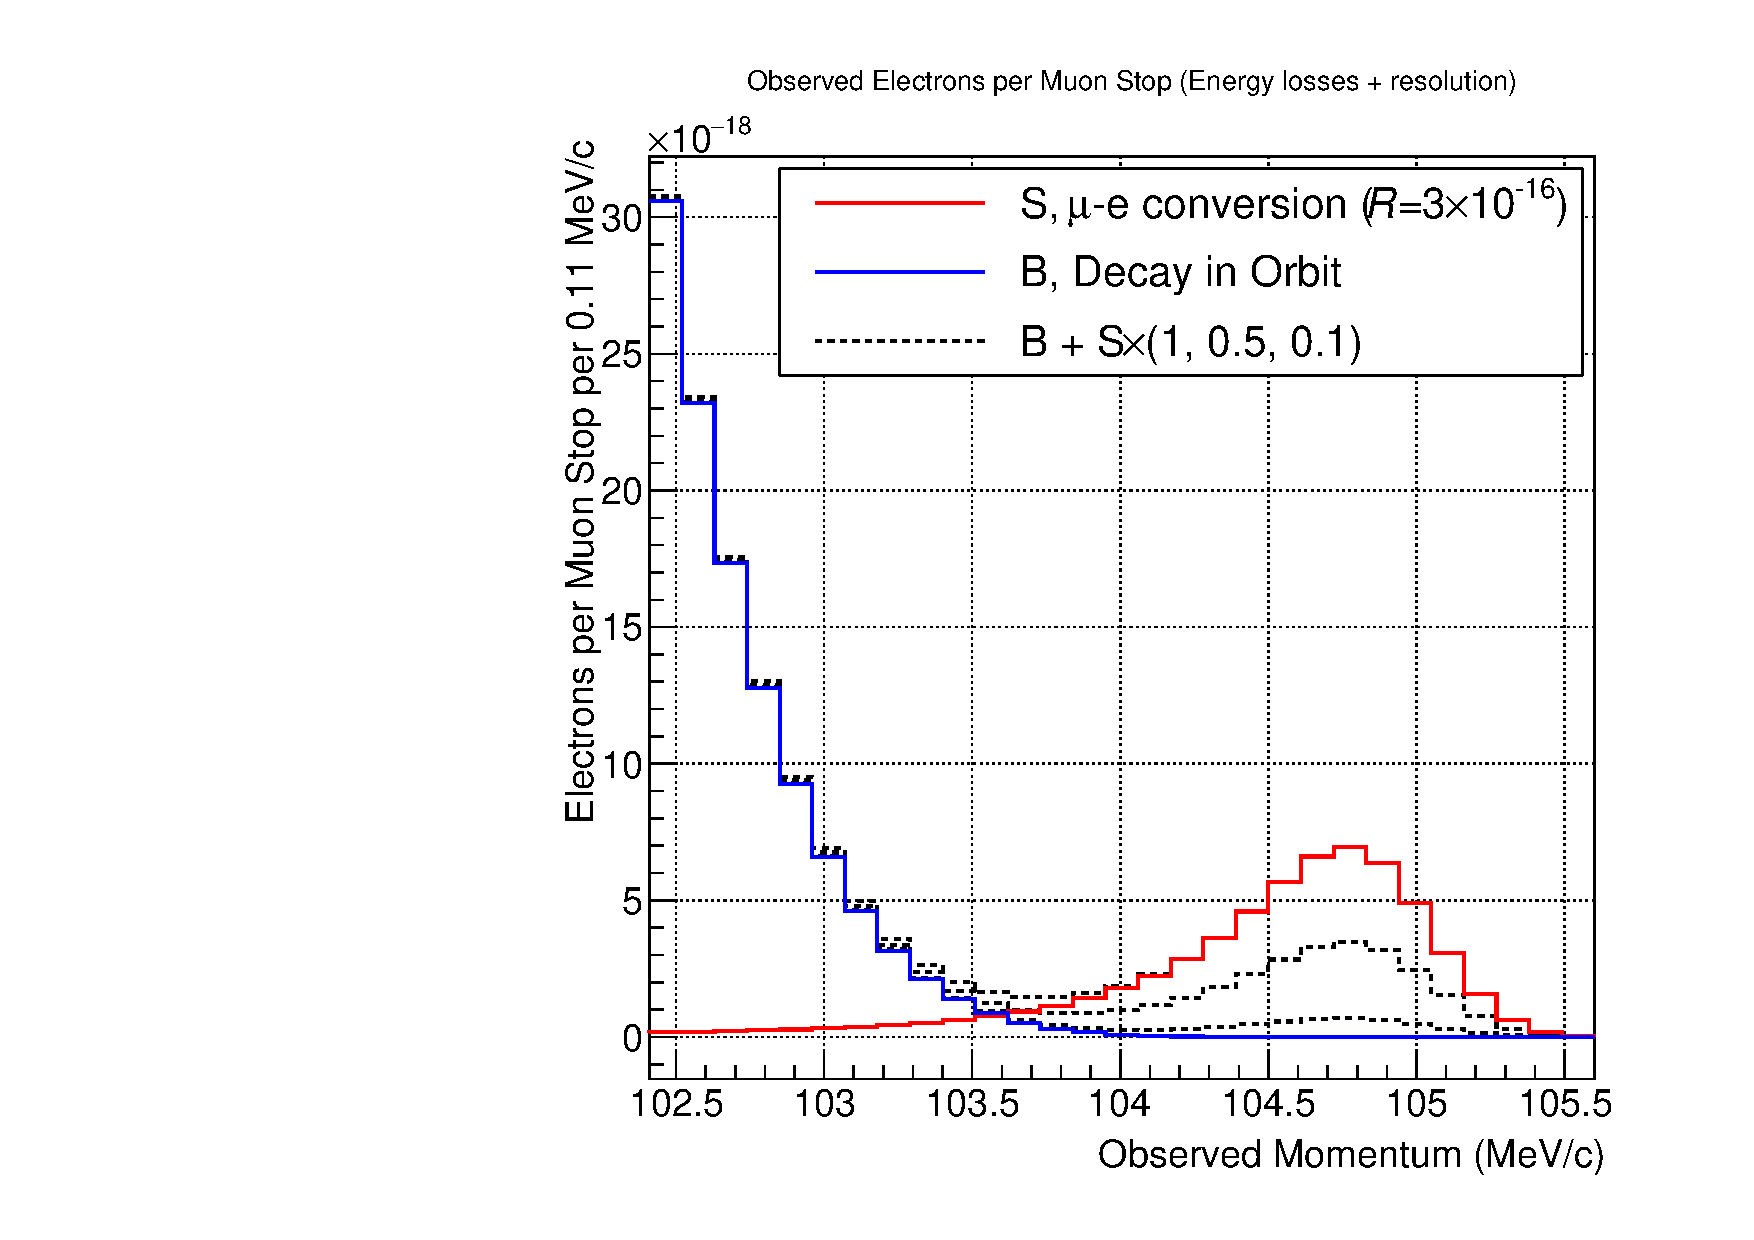
\includegraphics[width=0.48\textwidth,trim=0.0cm 0.0cm 1.0cm 1.0cm,clip]{figs/sensitivity/ConversionVsDio_Spectra-wResolution.pdf}}
\caption{\figlabel{optim:sense:spectra}
The spectrum of electrons coming from \ac{DIO} and \mueconv assuming a conversion rate of $\mathcal{R}=\sci{3}{-16}$.
\protect\subref{fig:optim:sense:spectra:ELoss} Includes energy losses in the target, beamline, and detector;
\protect\subref{fig:optim:sense:spectra:resolution} also includes resolution effects (assumed the resolution function is perfect gaussian with a width of $\sigma=200$~keV/c).
}
\end{figure}
}

\newcommand{\FigSensMomIntegral}{
\begin{figure}[tb]
\centering 
%\fbox{
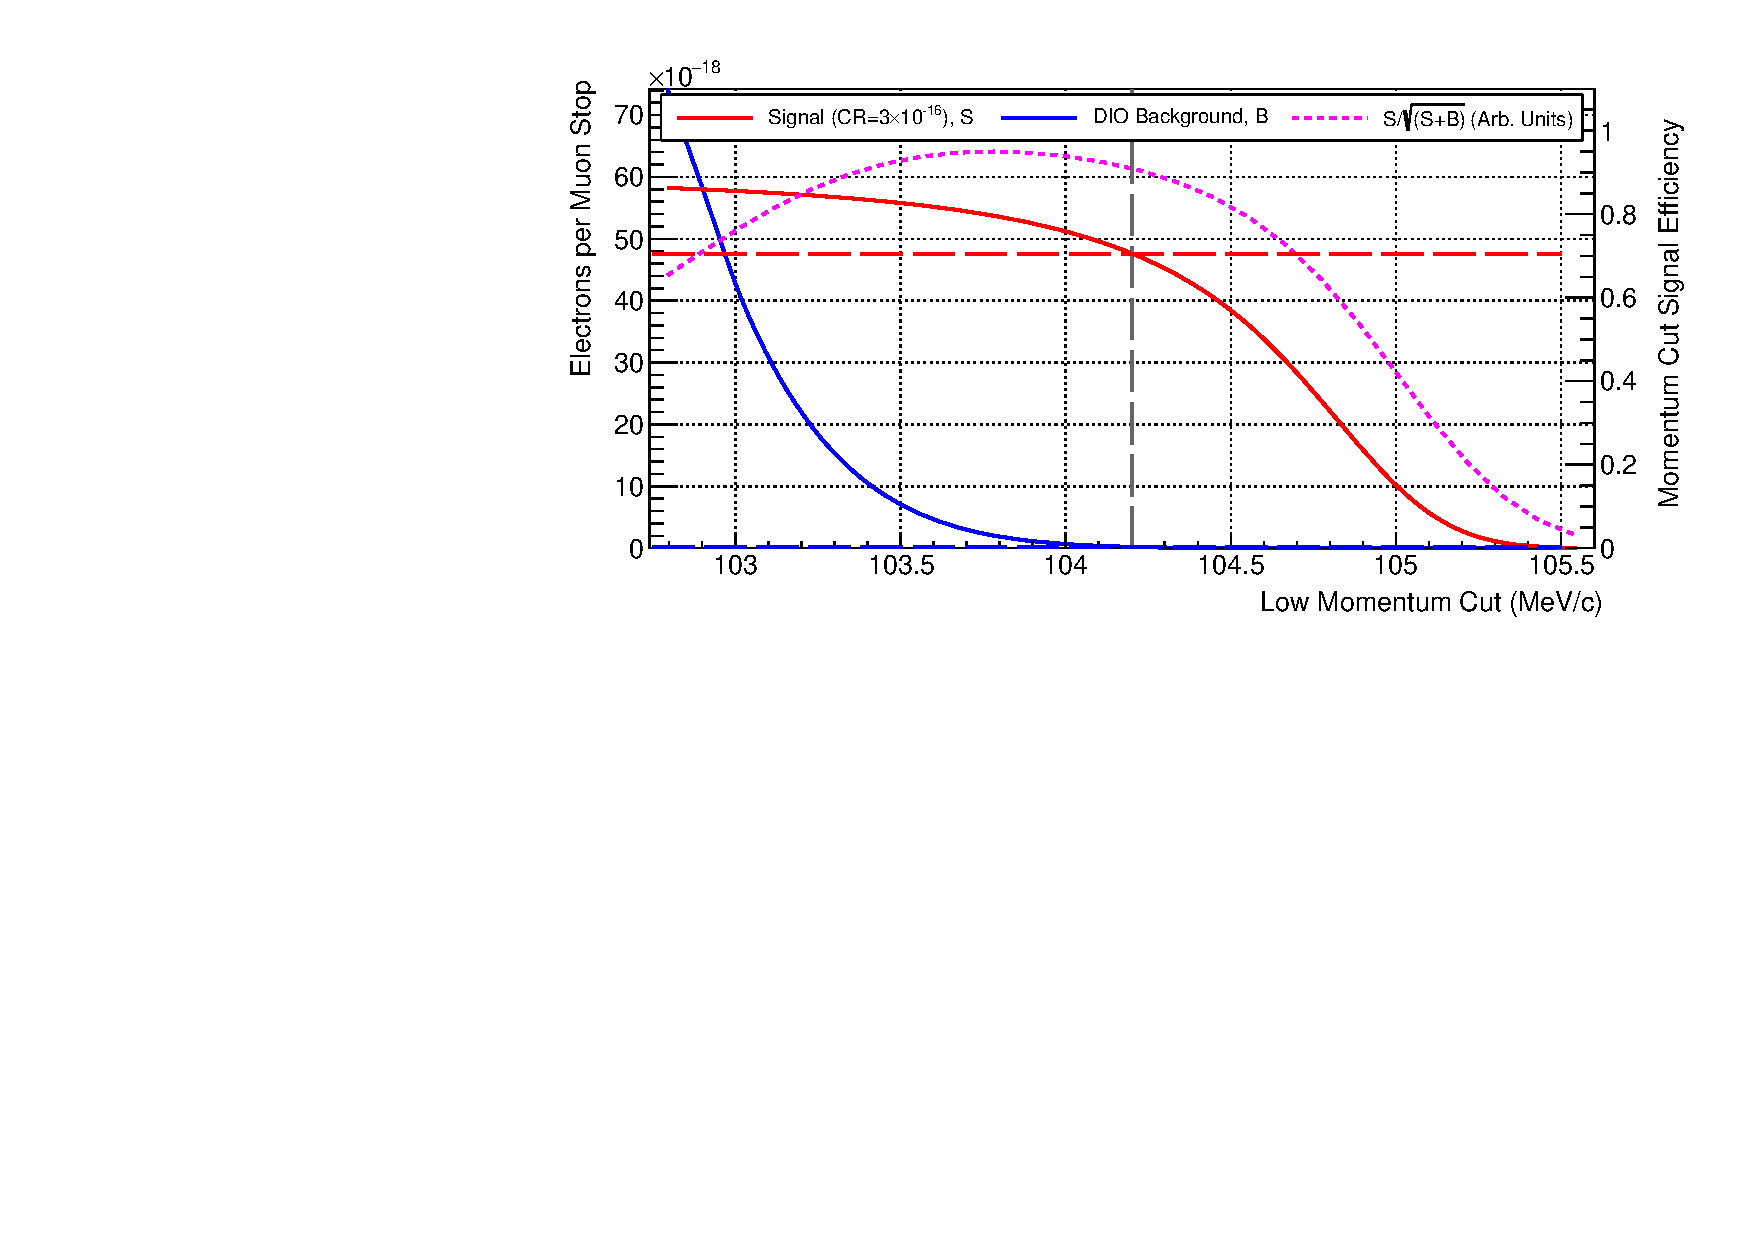
\includegraphics[width=0.99\textwidth,trim=1.0cm 0.0cm 1.0cm 0.6cm,clip]{figs/sensitivity/ConversionVsDio_Integrated.pdf}
%}
\caption{\figlabel{optim:sense:integral}
Relative signal versus \ac{DIO} background as a function of the low momentum cut value assuming a conversion rate of $\mathcal{R}=\sci{3}{-16}$.
The magenta line is the signal over square root of signal plus background for this conversion rate shown as an indicator of the optimum cut value.
}
\end{figure}
}

\newcommand{\FigSensTiming}{
\begin{figure}[tb]
\centering 
%\fbox{
\subfloat[\figlabel{optim:sense:timing:signal}Signal Arrival Time]      {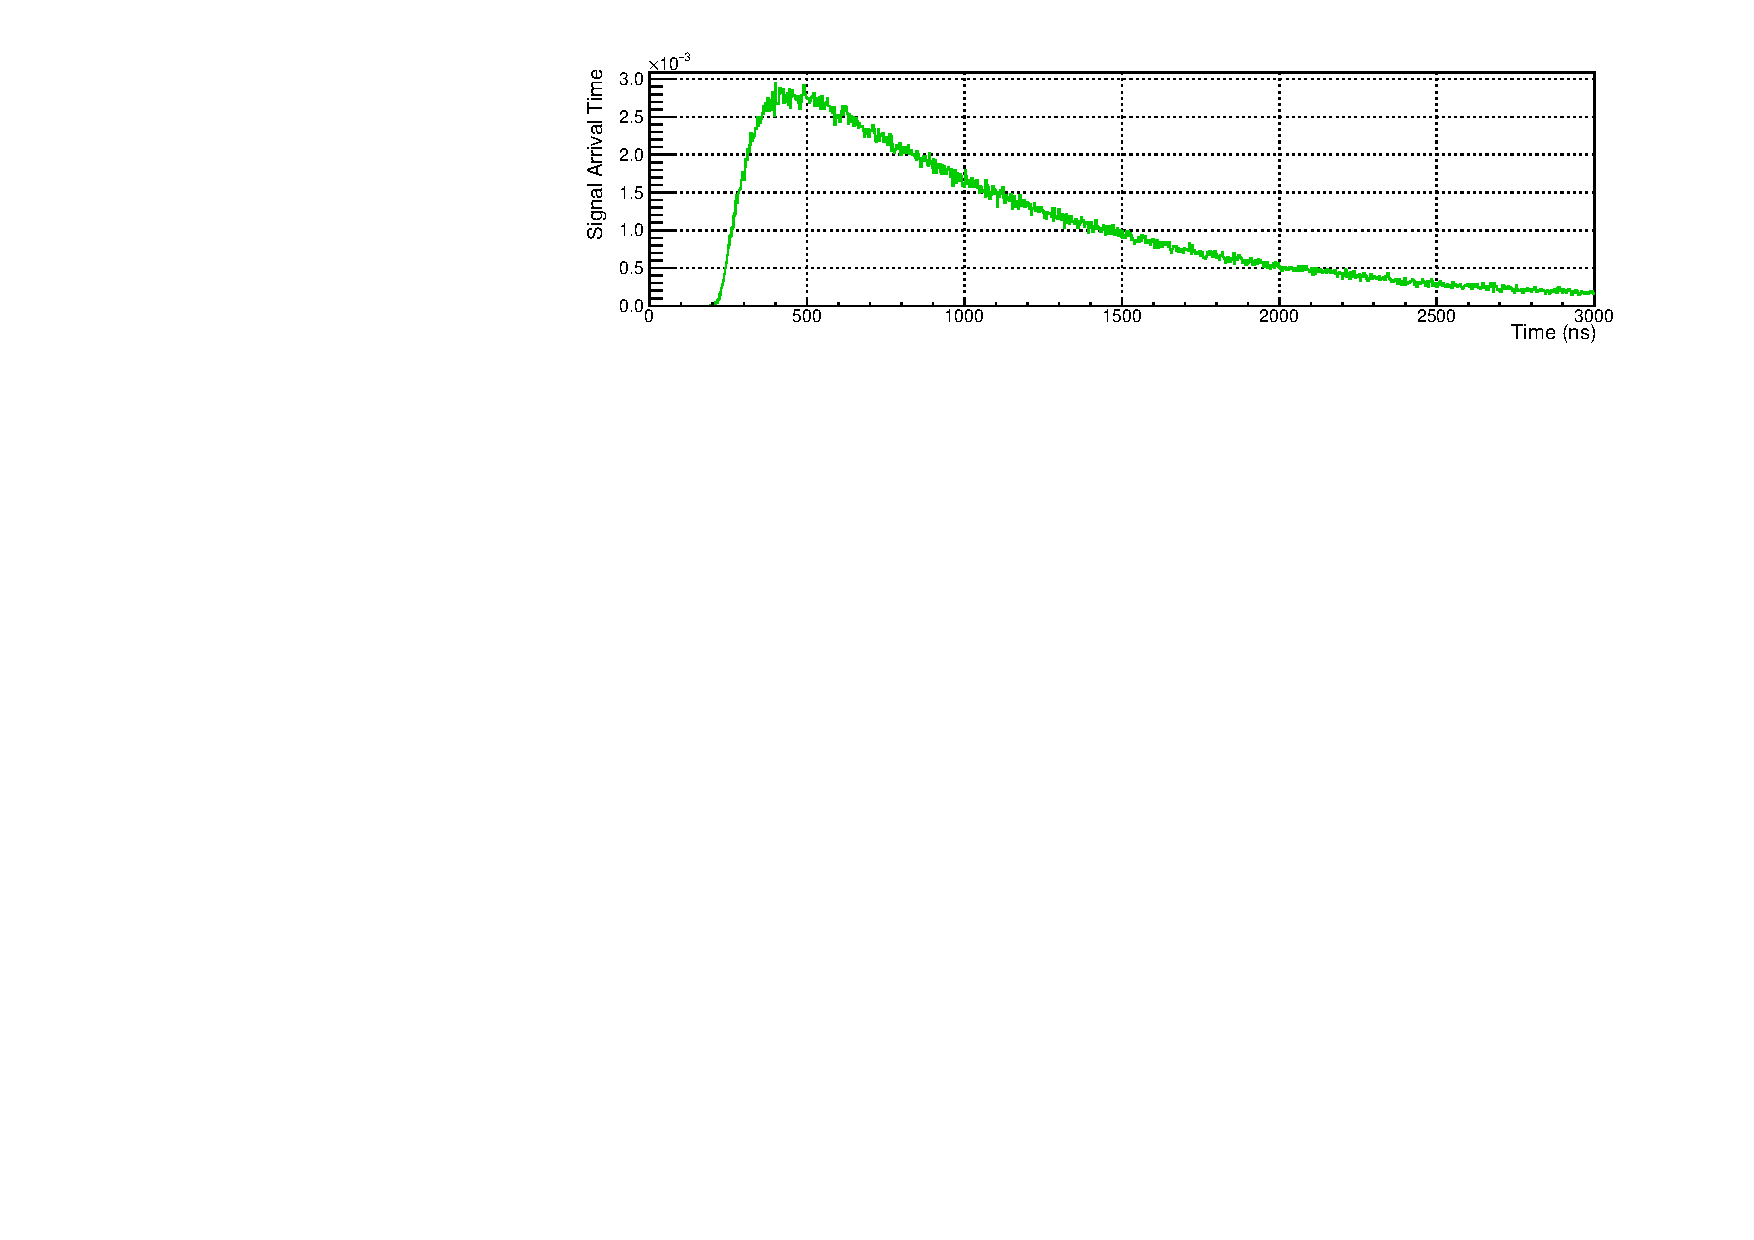
\includegraphics[width=0.9\textwidth,trim=0.9cm 0.1cm 1.5cm 0.20cm,clip]{figs/sensitivity/160823_MuonLifetime.pdf}}\\
\subfloat[\figlabel{optim:sense:timing:efficiency}Timing Cut Efficiency]{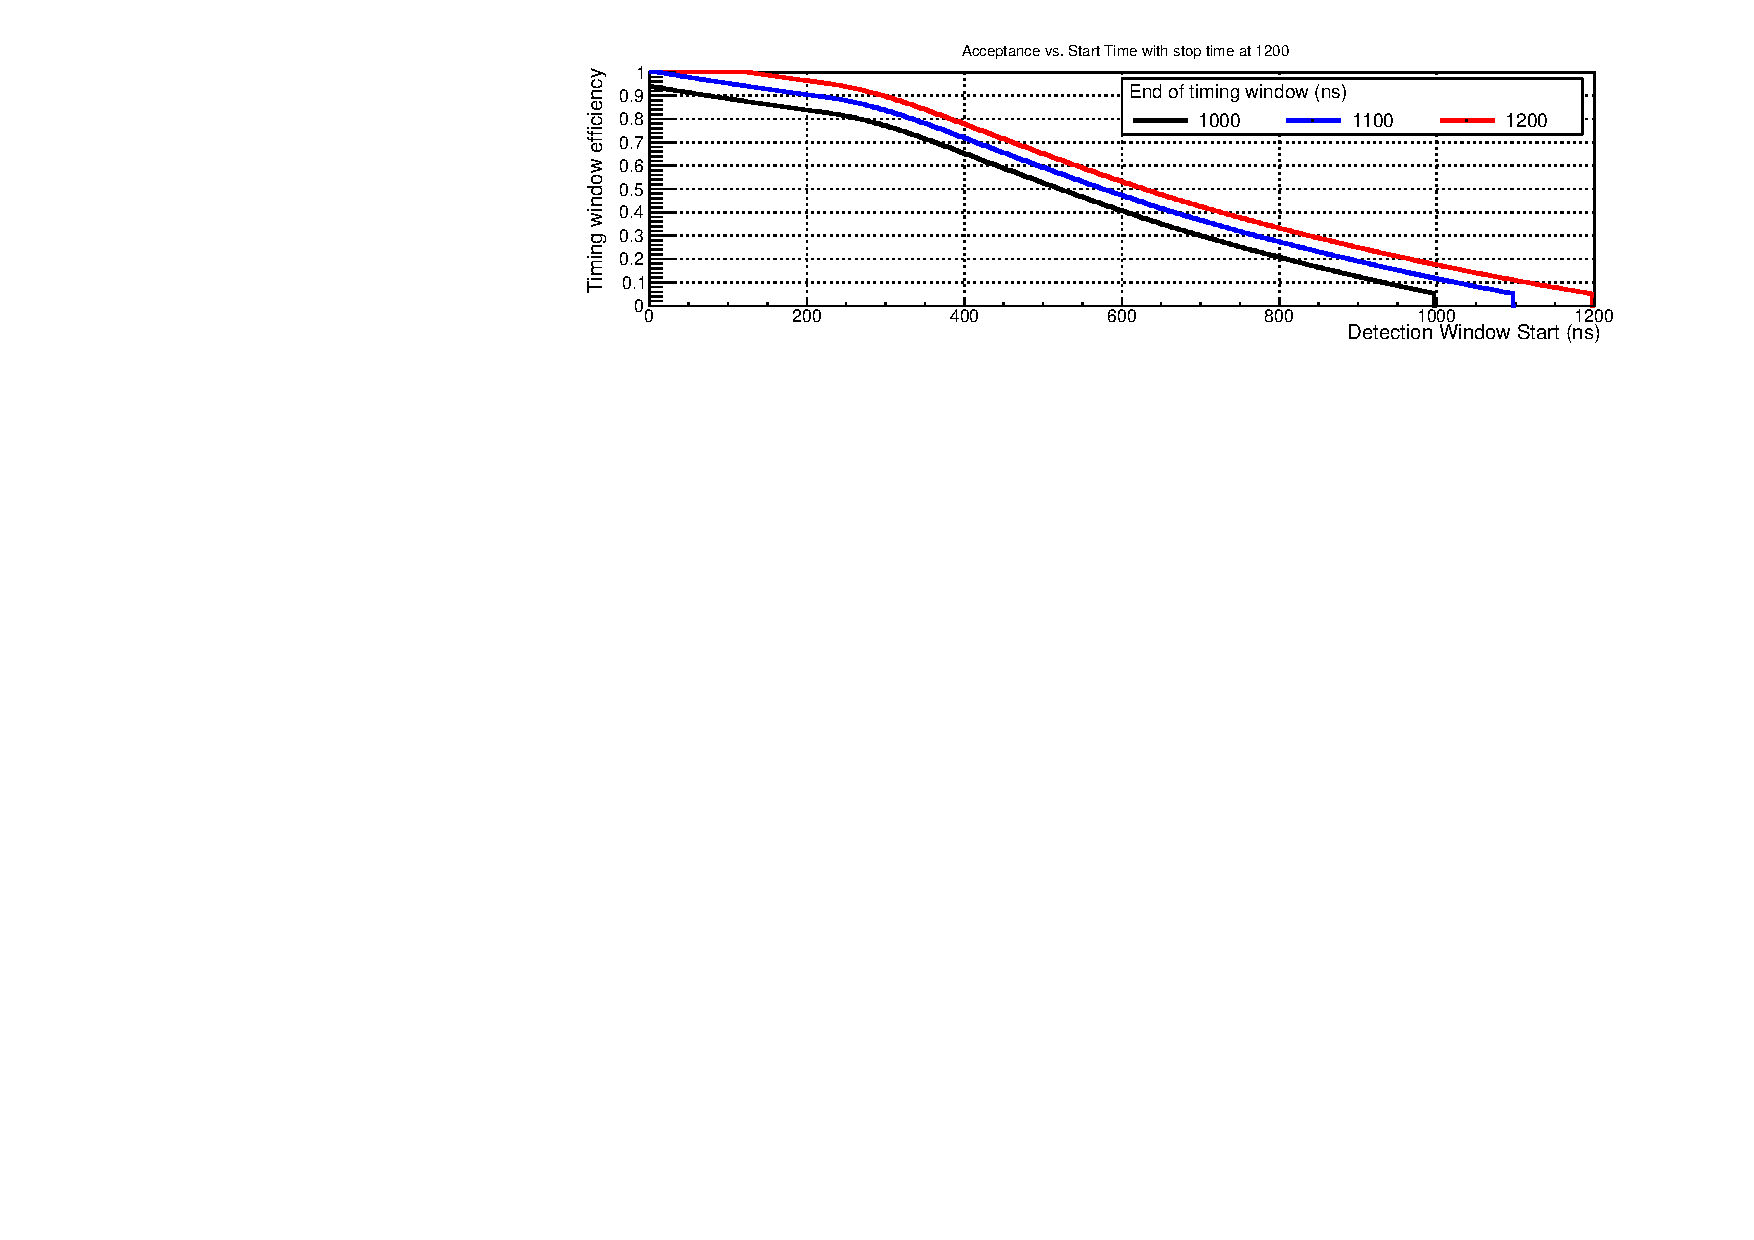
\includegraphics[width=0.9\textwidth,trim=0.9cm 0.1cm 1.5cm 0.4cm,clip]{figs/sensitivity/160823_TimingCutEfficiency.pdf}}
\caption{\figlabel{optim:sense:timing}
Timing of signal electrons.
\protect\subref{fig:optim:sense:timing:signal} The arrival time of signal electrons at the detector, including the effect of the proton pulse width, particle transportation, and the muon lifetime.
\protect\subref{fig:optim:sense:timing:efficiency} the efficiency of the timing window as a function of the switch-on time.  Assumes a pulse separation of 1.17~$\mu$s.
}
\end{figure}
}

